\setcounter{page}{1} \pagenumbering{Alph}

% Add PDF bookmark 
\pdfbookmark[0]{Title}{Title}

%%% LOGO
\thispagestyle{empty}
\begin{flushleft} ~\\ \vspace{-12mm} \hspace{-12mm}  
\includegraphics[width=50mm]{Cover/istnewlogo} 
 
 %%% Instituição
\centering
\LARGE \textbf{Universidade de Lisboa \\ Instituto Superior Técnico}
%%% espaço sem gráficos
\vspace{30mm}

%%% Optional Image
%\vspace{10mm}
%~\\ \vspace{50mm} % gráficos
%\\ \begin{center} 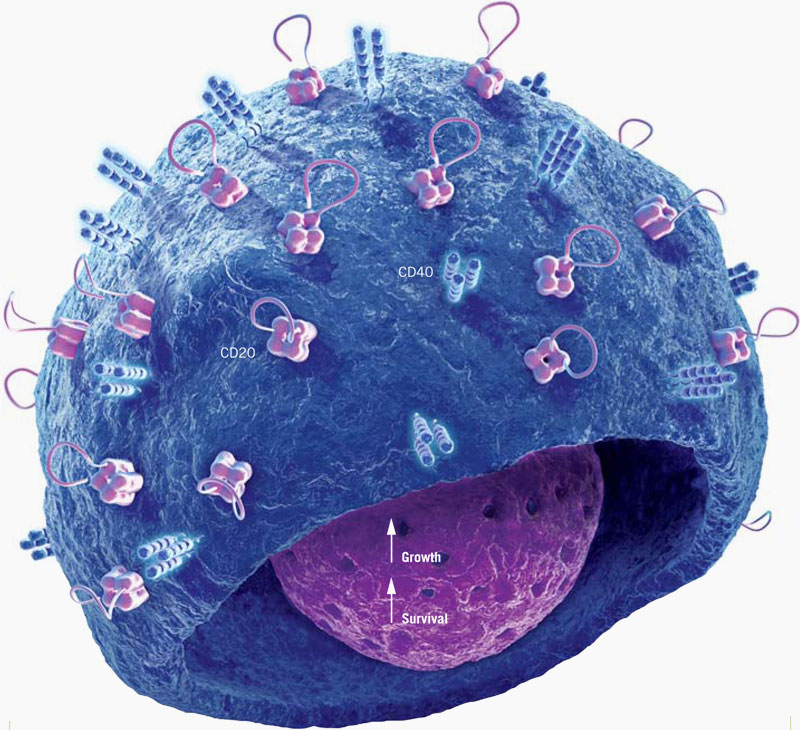
\includegraphics[height=50mm]{Cover/coverimage}  \end{center} % gráficos
 \vspace{5mm}
 
 %%% Titulo
\centering
\LARGE \textbf{Título da Tese que descreve o objeto de estudo.}
\\ \vspace{10mm}
\Large Subtítulo Opcional
\\ \vspace{15mm}
%\\ \vspace{25mm}  % NO SUBTITLE
\Large \textbf{Nome completo} \\
\vspace{4cm}

\begin{minipage}{\textwidth}
\begin{tabularx}{\textwidth}{ l @{ } l }
\large \textbf{Orientador} : & \textbf{Doutor} Nome completo\\
 \large \textbf{Co-Orientador} :  & \textbf{Doutor} Nome completo\\
 %&    ~~~~~~~~~~~~~~~~~~~~~~~~~~ large name\\
\end{tabularx}

\end{minipage}
%
\\ \vspace{27mm}
%\vspace{12mm}
\centering
\large \textbf{Tese especialmente elaborada para a obtenção do grau de Doutor em}\\
\large Engenharia Mecânica\\
%\\ \vspace{2mm}
\vspace{18mm}
\Large \textbf{Tese Provisória}
 
\vspace{15mm}

%\large \textbf{\todaythesis\today} \\
\large \textbf{November 2017} \\
\let\thepage\relax
\end{flushleft}
\pagebreak
